\documentclass[usenames,dvipsnames,notes]{beamer}
\usepackage{ifthen}
\usepackage{xcolor}
\usepackage{pgfplots}
\usepackage{amsmath}
\usepackage{centernot}
\usepackage{pifont}
\usepackage{tabularx}
\usepackage{makecell}
\usepackage{cuted}
\usepackage{booktabs}
\usepackage{array}

\usepackage{pgfpages}
%\setbeameroption{show notes on second screen}


\input ../beamer-style
\input ../std-macros
\input ../macros

\AtBeginSection[]
{
    \begin{frame}
        \frametitle{Table of Contents}
        \tableofcontents[currentsection]
    \end{frame}
}
\parskip=10pt

\title[CSCI-GA.2590]{Distributed representation of text}
\author[He He]{He He
}
\institute[NYU]{New York University}
\date{\today}

\begin{document}
\begin{frame}
\titlepage
\end{frame}

\begin{frame}
    {Logistics}
    Fix errors in HW1:\\
    \begin{itemize}
        \item Question 2.2
            $$
            \frac{d}{d\alpha}{\color{red}\log}\sigma(\alpha)
            $$
        \item Question 2.5
            $$
            p_N(w) {\color{red}\propto} p_{\text{unigram}}^\beta(w)
            $$
    \end{itemize}
\end{frame}

\section{Review}
\begin{frame}
    {Last week}
    Generative vs discriminative models for text classification\\
    \begin{itemize}
        \item (Multinomial) naive Bayes
            \begin{itemize}
                \item Assumes conditional independence
                \item Very efficient in practice (closed-form solution)
            \end{itemize}
        \item Logistic regression
            \begin{itemize}
                \item Works with all kinds of features
                \item Wins with more data
            \end{itemize}
    \end{itemize}

    Features for text\\
    \begin{itemize}
        \item BoW representation
        \item N-gram features (usually $n\le 3$)
    \end{itemize}

    Control the complexity of the hypothesis class\\
    \begin{itemize}
        \item Feature selection
        \item Norm regularization
        \item Hyperparameter tuning on the validation set
    \end{itemize}
\end{frame}

\begin{frame}
    {Evaluation}
    \begin{itemize}
        \itemsep3em
        \item Accuracy
        \item Precision
        \item Recall 
        \item F1
        \item Macro vs micro average
    \end{itemize}
\end{frame}

\section{Introduction}

\begin{frame}
    {Objective}    
    Goal: come up a \emph{good representation} of text\\
    \begin{itemize}
        \itemsep5em
        \item What is a representation?
        \item What is a good representation?
    \end{itemize}
    \vspace{3em}

\end{frame}

\begin{frame}
    {Distance functions}
    Let's check if BoW is a good representation.

    \textbf{Euclidean distance}\\
    \begin{itemize}
        \item[] For $a,b\in\BR^d$,
            $$
            d(a,b) = \sqrt{\sum_{i=1}^d(a_i-b_i)^2} \;.
            $$
        \item[] What if $b$ repeats each sentence in $a$ twice?
    \end{itemize}

    \pause
    \textbf{Cosine similarity}\\
    \begin{itemize}
        \item[] For $a,b\in\BR^d$,
            $$
            \text{sim}(a,b) = \frac{a\cdot b}{\norm{a}\norm{b}} = \cos\alpha
            $$
        \item[] Angle between two vectors
    \end{itemize}
\end{frame}

\begin{frame}
    {Example: information retrieval}
    Given a set of documents and a query,
    use the BoW representation and cosine similarity
    to find the most relevant document.

    What are potential problems?
    
    \vspace{5em}

    \pause
    Example:\\
    \begin{itemize}
        \item[] Q: Who \textcolor{blue}{has watched} \textcolor{red}{Tenet}?
        \item[] She \textcolor{blue}{has} just \textcolor{blue}{watched} Joker.
        \item[] \textcolor{red}{Tenet} was shown here last week.
    \end{itemize}
\end{frame}

\begin{frame}
    {TFIDF}
    \emph{Key idea}: upweight words that carry more information about the document

    Representation $\phi\colon \text{document} \rightarrow \BR^{|\sV|}$

    TFIDF:\\
    $$
    \phi_i(d) = \underbrace{\text{count}(w_i, d)}_{\text{term frequency}} \times
    \underbrace{\log \frac{\text{\# documents}}{\text{\# documents containing $w_i$}}}_{\text{inverse document frequency}}
    \;.
    $$

    Justification:\\
    $$
    \text{idf}(w, d) = \text{PMI}(w; d) = \log\frac{p(d\mid w)}{p(d)} \;.
    $$
\end{frame}

\section{Vector space models}

\begin{frame}
    {The distributional hypothesis}
    \nl{You shall know a word by the company it keeps.} (Firth, 1957)

    Word guessing!\\
    \begin{itemize}[<+->]
        \item[] Everybody likes \textcolor{blue}{tezg\"uino}.
        \item[] We make \textcolor{blue}{tezg\"uino} out of corn.
        \item[] A bottle of \textcolor{blue}{tezg\"uino} is on the table.
        \item[] Don't have \textcolor{blue}{tezg\"uino} before you drive.
    \end{itemize}

    \emph{Takeaway}: the meaning of a word can be representated by its neighbors.
\end{frame}

\begin{frame}
    {Choose the context}
    Where does the neighbors come from? (What relations are we interested in?)

    Construct a matrix where\\
    \begin{itemize}
        \item Row and columns represent two sets of objects (e.g. words)
        \item Each entry is the (adjusted) co-occurence counts of two objects
    \end{itemize}

    Example:\\
    \begin{itemize}
        \item words $\times$ documents
    \end{itemize}
    \vspace{7em}
\end{frame}

\begin{frame}
    {Reweight counts}
    Upweight informative words

    \textbf{Pointwise mutual information} (PMI)
    $$
    \text{PMI}(x;y) = \log \frac{p(x,y)}{p(x)p(y)}
    = \log\frac{p(x\mid y)}{p(x)}
    = \log\frac{p(y\mid x)}{p(y)}
    $$
    \vspace{-1em}
    \begin{itemize}
        \itemsep1em
        \item Symmetric: $\text{PMI}(x;y)=\text{PMI}(y;x)$
        \item Range: $(-\infty, \min(-\log p(x), -\log p(y)))$
        \item Estimates:
            \begin{align*}
            \hat{p}(x\mid y) = \frac{\text{count}(x,y)}{\text{count}(y)}\quad
            \hat{p}(x) = \frac{\text{count}(x)}{\sum_{x'\in\sX}\text{count}(x')}
            \end{align*}
        \item $\text{PPMI}(x;y) \eqdef \max(0, \text{PMI}(x;y))$
    \end{itemize}
\end{frame}

\begin{frame}
    {Dimensionality reduction}
    \emph{Motivation}: want a lower-dimensional, dense representation for efficiency

    Recall \textbf{SVD}: given a $m\times n$ matrix $A_{m\times n}$,
    we can decompose it to
    $$
    U_{m\times m}\Sigma_{m\times n}V_{n\times n}^T \;,
    $$
    where $U$ and $V$ are orthogonal matrices, and $\Sigma$ is a diagonal matrix.

    \emph{Interpretation}: consider the largest singular value $\sigma_1$,
    $$
    Av_1 = \sigma_1 u_1 \;.
    $$
    \vspace{-2em}
    \begin{itemize}
        \item $u_1$ is a vector in the column space of $A$
        \item $u_1$ is the direction where the column vectors vary the most
    \end{itemize}
\end{frame}

\begin{frame}
    {SVD for the word-document matrix}
\end{frame}

\begin{frame}
    {Summary}
    \textbf{Vector space models}\\
    \begin{enumerate}
        \item Design the matrix, e.g. word $\times$ document, people $\times$ movie.
        \item Reweight the raw counts, e.g. TFIDF, PMI.
        \item Reduce dimensionality by (truncated) SVD.
        \item Use word/person/etc. vectors in downstream tasks.
    \end{enumerate}
    
    \emph{Key idea}:\\
    \begin{itemize}
        \item Represent an object by its connection to other objects in the data.
        \item For NLP, the word meaning can be represented by the context it occurs in.
    \end{itemize}
\end{frame}

\section{Word embeddings}

\begin{frame}
    {Learning word embeddings}
    \emph{Goal}: map each word to a vector in $\BR^d$ such that \textit{similar} words also have \textit{similar} word vectors.
    \vspace{1em}

    Can we formalize this as a prediction problem?\\
    \begin{itemize}
        \item Needs to be self-supervised since our data is unlabeled.
        \item Low error $\implies$ similar words have simliar representations.
    \end{itemize}
    \vspace{1em}

    Intuition: word guessing\\
    \begin{itemize}
        \item Predict a word based on its context
        \item Predict the context given a word
    \end{itemize}
\end{frame}

\begin{frame}
    {The skip-gram model}
    \emph{Task}: given a word, predict its neighboring words within a window
    \begin{center}
        The quick brown fox jumps over the lazy dog
    \end{center}

    Assume conditional independence of the context words:
    $$
    p(w_{i-k}, \ldots, w_{i-1}, w_{i+1}, \ldots, w_{i+k} \mid w_i) =
 \prod_{j=i-k}^{i-1}p(w_j\mid w_i)
    $$

    How to model $p(w_j\mid w_i)$?
\end{frame}

\begin{frame}
    {The skip-gram model}
    Use logistic regression\\
    \begin{align*}
        p(w_j\mid w_i) &= \frac{\exp\pb{\theta_{w_j}\cdot \phi(w_i)}}
    {\sum_{w\in\sV} \exp\pb{\theta_{w}\cdot\phi(w_i)}} \\\\
        &= \frac{\exp\pb{\phi_{\text{ctx}}(w_j)\cdot \phi_{\text{wrd}}(w_i)}}
        {\sum_{w\in\sV} \exp\pb{\phi_{\text{ctx}}(w_j)\cdot\phi_{\text{wrd}}(w_i)}} \\
    \end{align*}
    %
    \begin{itemize}
        \item $\phi\colon w \mapsto A_{d\times|\sV|}\phi_{\text{BoW}}(w)$
        \item In practice, $\phi$ is implemented as a dictionary
        \item Learn parameters by MLE and SGD (is the objective convex?)
        \item $\phi_{\text{wrd}}$ is taken as the word embedding
    \end{itemize}
\end{frame}

\begin{frame}
    {The continuous bag-of-words model}
    \emph{Task}: given the context, predict the word in the middle 
    \begin{center}
        The quick brown fox jumps over the lazy dog
    \end{center}

    Similary, we can use logistic regression for the prediction
    $$
    p(w_i \mid w_{i-k}, \ldots, w_{i-1}, w_{i+1}, \ldots, w_{i+k})
    $$

    How to represent the context (input feature)?
\end{frame}

\begin{frame}
    {The continuous bag-of-words model}
    \begin{align*}
        c &= w_{i-k}, \ldots, w_{i-1}, w_{i+1}, \ldots, w_{i+k} \\\\
        p(w_i\mid c) &= \frac{\exp\pb{\theta_{w_i}\cdot \phi_{\text{BoW}}(c)}}
        {\sum_{w\in\sV} \exp\pb{\theta_{w}\cdot\phi_{\text{BoW}}(c)}} \\\\
        &= \frac{\exp\pb{\phi_{\text{wrd}}(w_i)\cdot \sum_{w'\in c}\phi_{\text{ctx}}(w')}}
        {\sum_{w\in\sV} \exp\pb{\phi_{\text{wrd}}(w)\cdot\sum_{w'\in c}\phi_{\text{ctx}}(w')}} \\
    \end{align*}

    \begin{itemize}
        \item Implementation is similar to the skip-gram model.
    \end{itemize}
\end{frame}

\begin{frame}
    {Properties of word embeddings}
    \begin{itemize}
        \itemsep1em
        \item Find synonyms
        \item Solve word analogy problems
            \begin{itemize}
                \item[] man : woman :: king : queen
                \item[] $\phi_{\text{wrd}}(\text{man}) - \phi_{\text{wrd}}(\text{woman}) \approx \phi_{\text{wrd}}(\text{king}) - \phi_{\text{wrd}}(\text{queen})$
                \item[]
                \item[] man : woman :: king : ? 
                \item[] $\argmax_{w\in\sV} \text{sim}(-\phi_{\text{wrd}}(\text{man}) + \phi_{\text{wrd}}(\text{woman}) + \phi_{\text{wrd}}(\text{king}), w)$
            \end{itemize}
        \item[] [demo]
    \end{itemize}
\end{frame}

\begin{frame}
    {Comparison}
    \begin{table}
        \begin{tabular}{p{4cm}p{7cm}}
            vector space models & word embeddings \\
            \midrule
            matrix factorization & prediction problem \\
            fast to train & slow (with large corpus) but more flexible \\
            interpretable components & hard to interprete but has intriguing properties
        \end{tabular}

        Both uses the distributional hypothesis.
    \end{table}
\end{frame}

\begin{frame}
    {Summary}
    \emph{Key idea}: formalize word representation learning as a self-supervised prediction problem

    Prediction problems:\\
    \begin{itemize}
        \item CBOW: Predict word from context
        \item Skip-gram: Predict context from words
        \item Other possibilities:
            \begin{itemize}
                \item Predict $\log \hat{p} (\text{word}\mid \text{context})$, e.g. GloVe
                \item Contextual word embeddings
            \end{itemize}
    \end{itemize}

    Similar ideas can be used to learn embeddings of other objects, e.g. image, product etc.
\end{frame}

\section{Brown clusters}

\begin{frame}
    {Brown clustering}
    Developed at IBM by Peter Brown et al. in early 90s.

    \emph{Idea}: hierarchically clustering words (initially used for language modeling)
    
    \vspace{7em}
\end{frame}

\begin{frame}
    {Example clusters}
    \begin{figure}
        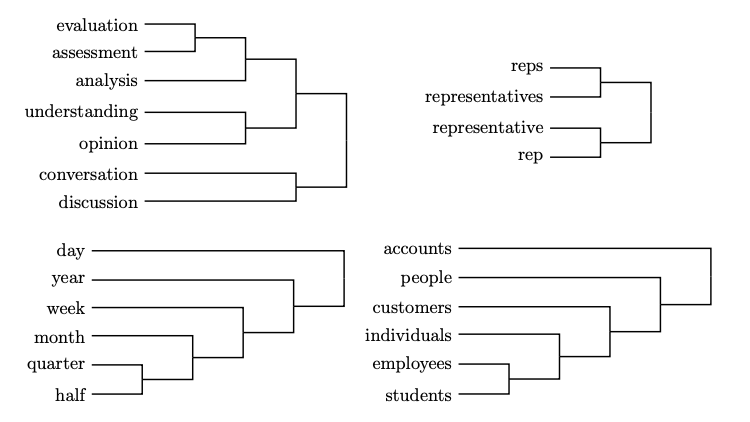
\includegraphics[width=12cm]{figures/brown-clusters}
    \end{figure}
\end{frame}

\begin{frame}
    {Bottom-up (agglomerative) clustering}
\end{frame}

\begin{frame}
    {Summary}
    Brown clustering\\
    \begin{enumerate}
        \item Obtain initial word representation
        \item Defind distance function between two clusters
        \item Run heirarchical clustering
        \item Use the (binary) ``path'' to a word as additional features in downstream tasks
    \end{enumerate}
\end{frame}

\begin{frame}
    {Evaluate word vectors}
    \textbf{Intrinsic evaluation}\\
    \begin{itemize}
        \item Evaluate on the proxy task (related to the learning objective)
        \item Word similarity/analogy datasets
        \item Human evaluation of word clusters
    \end{itemize}

    \textbf{Extrinsic evaluation}\\
    \begin{itemize}
        \item Evaluate on the real/downstream task we care about
        \item Use word vectors as features in NER, parsing etc.
    \end{itemize}
\end{frame}

\section{Neural networks and backpropogation}

\begin{frame}
    {Feature learning}
    Linear predictor with handcrafted features: $f(x) = w\cdot\phi(x)$.

    Can we learn intermediate features?

    Example:\\
    \begin{itemize}
    \item Predict popularity of restaurants.
    \item Raw input: \#dishes, price, wine option, zip code, \#seats, size 
    \item Decompose into subproblems:
    \begin{itemize}
        \itemsep2ex
    \item[] ${\color{blue}h_1}(\pb{\text{\#dishes, price, wine option}}) = \text{food quality}$
    \item[] ${\color{blue}h_2}(\pb{\text{zip code}}) = \text{walkable}$
    \item[] ${\color{blue}h_3}(\pb{\text{\#seats, size}}) = \text{nosie}$
    \end{itemize}
    \end{itemize}

\end{frame}

\begin{frame}
    {Learning intermediate features}
\begin{center}
\def\layersep{2.5cm}
\begin{tikzpicture}[shorten >=1pt,->,draw=black!50, node distance=\layersep]
    \tikzstyle{every pin edge}=[<-,shorten <=1pt]
    \tikzstyle{neuron}=[circle,fill=black!25,minimum size=17pt,inner sep=0pt]
    \tikzstyle{input neuron}=[neuron, fill=green!50];
    \tikzstyle{output neuron}=[neuron, fill=red!50];
    \tikzstyle{hidden neuron}=[neuron, fill=blue!50];
    \tikzstyle{annot} = [text width=4em, text centered]

    % Draw the input layer nodes
    \foreach \name / \y / \text in {1/1/\#dishes, 2/2/price, 3/3/wine option, 4/4/zip code, 5/5/\#seats, 6/6/size}
    % This is the same as writing \foreach \name / \y in {1/1,2/2,3/3,4/4}
        \node[input neuron, pin=left:\text] (I-\name) at (0,-\y) {};

    % Draw the hidden layer nodes
    \foreach \name / \y in {1,...,3}
        \path[yshift=-1.3cm]
            node[hidden neuron] (H-\name) at (\layersep,-\y cm) {};

    % Draw the output layer node
    \node[output neuron,node distance=4cm,pin={[pin edge={->}]right:Popularity}, right of=H-2] (O) {};

    % Connect every node in the input layer with every node in the
    % hidden layer.
    \foreach \source in {1,...,6}
        \foreach \dest in {1,...,3}
            \path (I-\source) edge (H-\dest);

    % Connect every node in the hidden layer with the output layer
    \foreach \source in {1,...,3}
        \path (H-\source) edge (O);

    % Annotate the layers
    \node[annot,above of=H-1, node distance=2.5cm] (hl) {\textcolor{blue}{Hidden} layer};
    \node[annot,left of=hl] {Input layer};
    \node[annot,right of=hl, node distance=4cm] {Output layer};
    
    % Annotate the hidden nodes
    \foreach \h / \text in {1/food quality, 2/walkable, 3/noise}
    		\node[annot, above of=H-\h, node distance=0.5cm] {$h_\h$};
\end{tikzpicture}
\end{center}
\end{frame}

\begin{frame}
    {Neural networks}
\emph{Key idea}: automatically learn the intermediate features.

    \textbf{Feature engineering}:
Manually specify $\phi(x)$ based on domain knowledge and learn the weights:
\begin{align*}
f(x) = {\color{red}w}^T\phi(x) .
\end{align*}

    \textbf{Feature learning}:
Automatically learn both the features ($K$ hidden units) and the weights:
\begin{align*}
h(x) = \pb{{\color{red}h_1}(x), \ldots, {\color{red}h_K}(x)} , \quad
f(x) = {\color{red}w}^T h(x)
\end{align*}

Parametrize $h$: $x \mapsto \sigma(v_i^T x)$.
\end{frame}

\end{document}
